\chapter{继电接触器控制系统}
\Par 如图\ref{fig:控制电路}所示,这是一个完整的控制系统下面的M表示\textbf{电机(Machine)},首先我们设计了一个\textbf{总闸开关Q},只要它断开,电机就一定启动不了.然后为了保护电路,我们添加了\textbf{熔断器(Fuse)FU},它可以在低压电路短路的时候断开来保护电路.如果只有总闸开关Q,就会导致两个问题,第一个是开关内部在断开时会产生电弧,因为电压太大了,这很危险;第二个是它总是常开或常闭,如果停电后突然来电,机器在总闸开关联通的时候会自动开机,这很危险.

\begin{figure}[htbp]
	\centering
	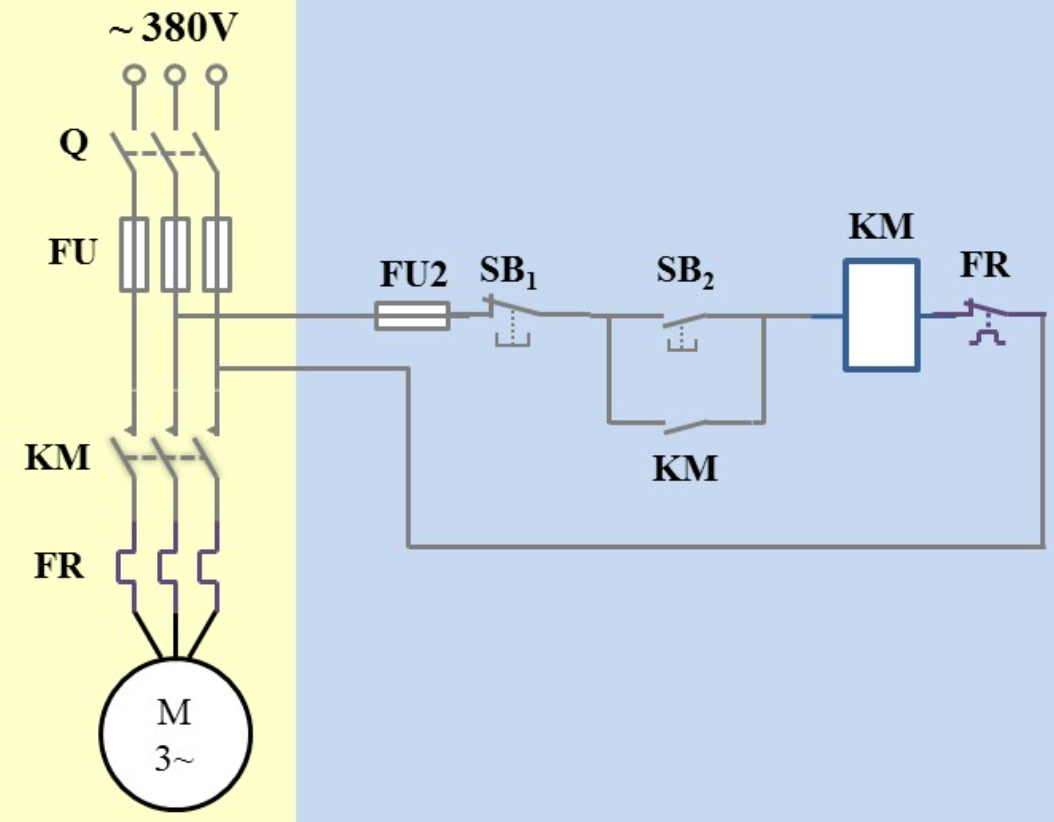
\includegraphics[width=0.65\textwidth]{控制电路.png}
	\caption{控制电路}
	\label{fig:控制电路}
\end{figure}
\Par 为此,我们安装了\textbf{交流接触器(Kontakte Motor)}KM,它利用电磁铁实现回路的开关,一按常开\textbf{按钮(Stop Button)}SB$_2$就会开启电机,松开就会断开电机,当然,它是需要电源接到电磁铁上的,就近我们选取电机的电源作为他的电源.如图中左侧三个标有KM的开关所示,这是交流接触器的\textbf{主触点},而右图中标有KM的小方块表示\textbf{电磁铁}.

\Par 右边那个标有KM的开关是它的\textbf{辅助触点},它并联在SB$_2$两边,它的存在是为了满足一项需求:如果我按住KM电机才能运行,那也太麻烦了!我想一键开关!当然,这不能像总闸开关一样,它要解决总闸开关的问题.当我们按下按钮SB$_2$时,KM所有的开关都会联通,这时,辅助触点也会联通,如果我们断开SB$_2$这时KM也不会断开,这就实现了电机的连续运行.

\Par 现在的问题是,你连续运行了要怎么结束呢?为此,我们安装常闭按钮SB$_1$,一按它就断开了.同时我们为这个电路安装上保护装置:\textbf{热继电器}FR,它的作用是过载保护,当点击长期高功率运行时会积累大量的热量,FR由双金属片和开关组成,当温度过高时,双金属片弯曲会使开关断开.
\begin{figure}[htbp]
	\centering
	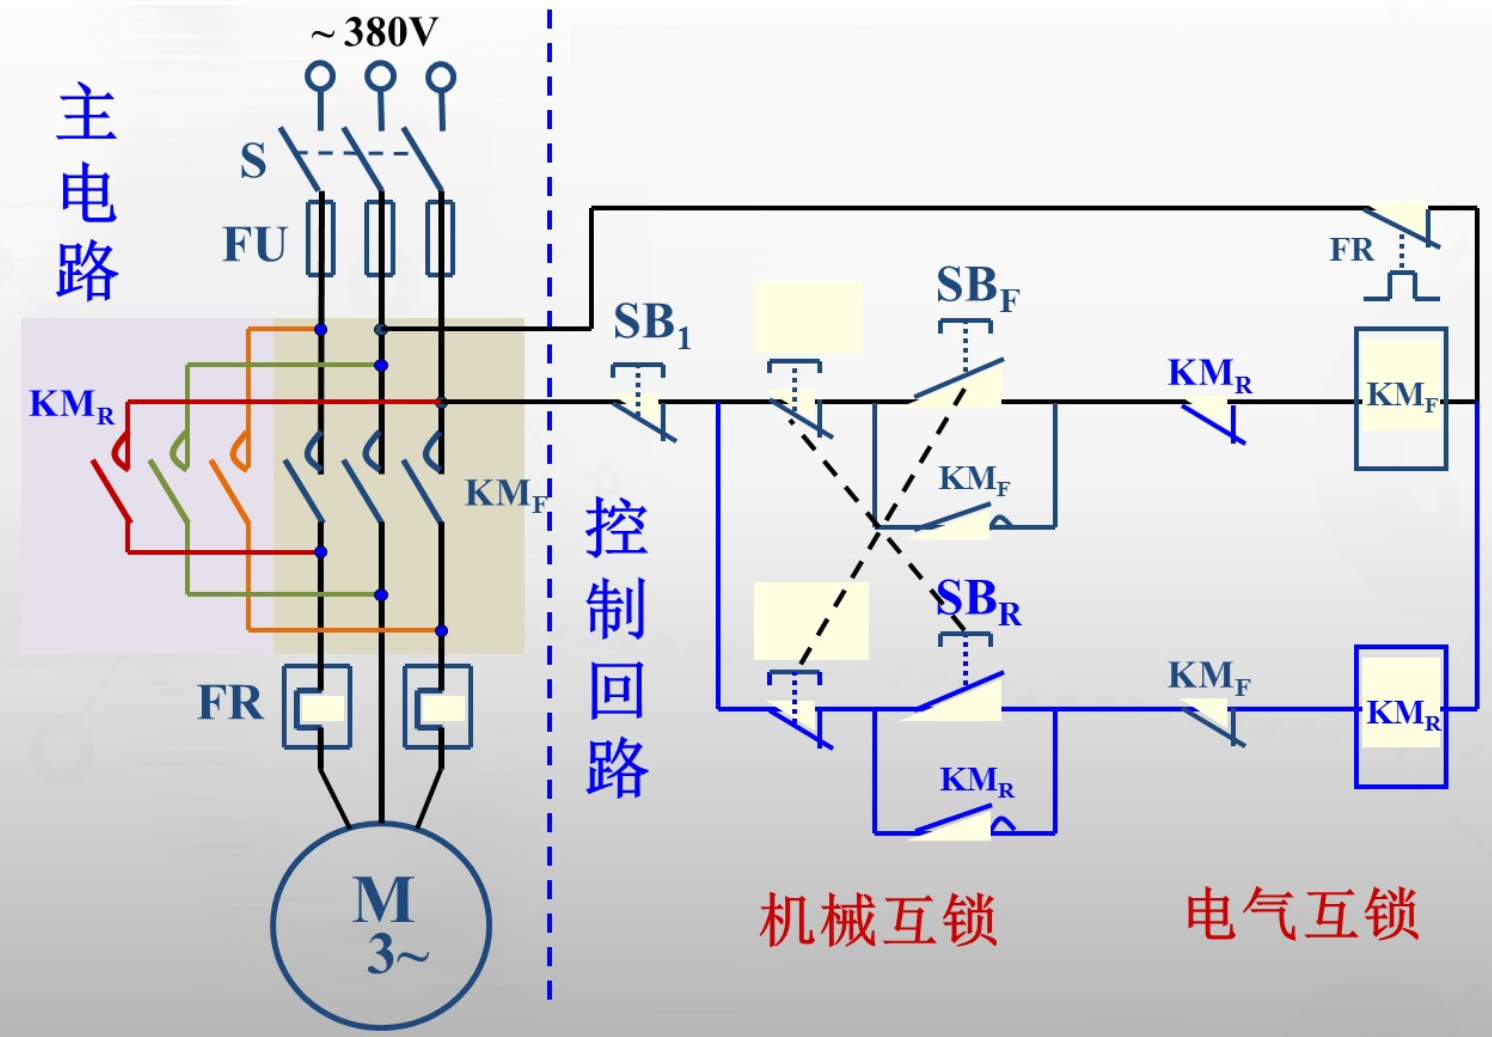
\includegraphics[width=0.65\textwidth]{正反转控制电路.png}
	\caption{正反转控制电路正反转控制电路}
	\label{fig:正反转控制电路}
\end{figure}

\Par 为了实现电机的正反转,我们安装上正反转控制电路,它让原来的三相交流电分别接到不同的电动机的电极上,同时采用了另一套与之前完全相同的继电控制系统.同样为了简化操作,让系统1的停止按钮SB$_1$与系统2的启动按钮SB$_\mathrm{R}$机械互锁,让系统2的停止按钮SB$_3$与系统1的启动按钮SB$_\mathrm{L}$机械互锁,当其中一个启动按钮被按下时,另一个系统的停止按钮在机械互锁的帮助下会先被按下,然后启动按钮再被按下,这样就不必先按下停止按钮再按反转按钮了.


